% =====================================================================
%  A Cut Invariant for Canonical Atom Ranking
%
%  Self-contained.  Every construction is defined here.
% =====================================================================
\documentclass[11pt,twocolumn,a4paper]{article}

\usepackage[utf8]{inputenc}
\usepackage[T1]{fontenc}
\usepackage{lmodern}
\usepackage[a4paper,margin=2.4cm]{geometry}
\usepackage{amsmath,amssymb,amsthm,mathtools}
\usepackage{bm}
\usepackage{booktabs}
\usepackage{array}
\usepackage{longtable}
\usepackage{enumitem}
\usepackage{microtype}
\usepackage{xcolor}
\usepackage{graphicx}
\usepackage[round,sort&compress]{natbib}
\usepackage[colorlinks=true,linkcolor=blue!45!black,
            citecolor=blue!45!black,urlcolor=blue!45!black]{hyperref}
\usepackage{cleveref}

\newtheoremstyle{crthm}{\topsep}{\topsep}{\itshape}{}{\bfseries}{.}{.5em}{}
\theoremstyle{crthm}
\newtheorem{theorem}{Theorem}[section]
\newtheorem{lemma}[theorem]{Lemma}
\newtheorem{proposition}[theorem]{Proposition}
\newtheorem{corollary}[theorem]{Corollary}
\theoremstyle{definition}
\newtheorem{definition}[theorem]{Definition}
\newtheorem{algorithmx}[theorem]{Algorithm}
\newtheorem{example}[theorem]{Example}
\theoremstyle{remark}
\newtheorem{remark}[theorem]{Remark}

\newcommand{\R}{\mathbb{R}}
\newcommand{\N}{\mathbb{N}}
\newcommand{\Gph}{\Gamma}
\newcommand{\V}{V}
\newcommand{\E}{E}
\newcommand{\wt}{w}
\newcommand{\med}{\mathsf{m}}
\newcommand{\cut}{\partial}
\newcommand{\sep}{\sigma}
\newcommand{\dep}{d}
\newcommand{\key}{\kappa}
\newcommand{\abs}[1]{\lvert#1\rvert}
\newcommand{\Aut}{\operatorname{Aut}}
\newcommand{\orb}{\mathcal{O}}

\title{\textbf{A Cut Invariant for Canonical Atom Ranking}\\[6pt]
\large Separation Cost, Burial Depth, and Refinement to the\\
Automorphism Partition}

\author{%
Kundai Farai Sachikonye\\[0.3em]
\normalsize Experimental Bioinformatics, TUM School of Life Sciences\\
\normalsize AIMe Registry for Artificial Intelligence \\
\normalsize Maximus-von-Imhof-Forum 3, 85354 Freising, Germany\\
\normalsize \texttt{kundai.sachikonye@bitspark.com}}

\date{\today}

\begin{document}
\maketitle

\tableofcontents

\begin{abstract}
\noindent
Canonical atom ranking underlies structure identity, canonical line
notation, and circular fingerprinting. The dominant family of methods
derives from Morgan's extended-connectivity algorithm: assign each atom a
label from its element and degree, iteratively replace that label by a
function of its neighbours' labels, and break the ties that remain by a
rule. The labels such a procedure produces are \emph{conventions}: they
are well defined and reproducible, but they are functions of the tie-break
rule as much as of the molecule, and nothing internal to the procedure
distinguishes two atoms that are genuinely equivalent from two that the
rule happened to separate.

We define an atom label that is not a convention. Each atom is assigned
the \emph{cut key} $\key(v)=(\sep(v),\dep(v))$: the minimum weight of a
cut separating $v$ from a distinguished medium vertex in a weighted
contact graph, together with the number of atoms on the minimising side.
Both are invariants of the weighted graph, computed by maximum flow rather
than by a hashing convention. We prove that the cut key is preserved by
every weighted isomorphism (\Cref{thm:invariance}), that iterating it
under neighbour refinement remains an invariant at every round
(\Cref{thm:refine-invariant}), and that the refinement is bounded below by
the orbit partition of the automorphism group and therefore never
separates two atoms that a symmetry of the molecule exchanges
(\Cref{thm:orbit-bound}). This is the property a canonical \emph{ordering}
does not have and cannot have, since an ordering must break every tie.

We report a validation suite whose expectations were registered in the
experiment source before it was run. On an eighteen-molecule corpus with
independently determined heavy-atom orbit counts, the refinement recovers
the orbit count exactly in $18/18$ cases, over-separating in none, with a
median of $2$ rounds. On a thirty-molecule drug-like corpus the base cut
key is coarse---mean distinct-key ratio $0.508$---and refinement raises it
to $0.827$, so neither the base invariant alone nor refinement alone is
the whole construction. A negative control that breaks ties by atom index,
which is what an ordering does, over-separates on $16$ of the $18$
symmetric molecules, confirming that the orbit agreement is not vacuous.

We state the limitations plainly. The construction is an invariant, not a
canonical form: it does not produce a total order and cannot be used
directly as a canonical labelling. Its refinement is a colour refinement
and inherits that family's known incompleteness on strongly regular
graphs. It is more expensive than Morgan by a factor of the maximum-flow
cost. And the corpus is small and hand-assembled. What the construction
provides is a label whose equality is a fact about the molecule rather
than about the labelling procedure, together with the burial depth, a
quantity the conventional atom identifier does not carry.
\end{abstract}

\noindent\textbf{Keywords:} canonical ranking; atom invariant; minimum
cut; colour refinement; automorphism orbits; circular fingerprints;
molecular symmetry.

\tableofcontents

% =====================================================================
\section{Introduction}
\label{sec:intro}
% =====================================================================

\subsection{What a canonical ranking is for}

Many cheminformatics operations require the atoms of a structure to be
put in a definite order. Canonical line notations need one so that the
same molecule always yields the same string \citep{weininger1989}.
Structure-identity comparison needs one, or an equivalent invariant, to
decide whether two connection tables describe the same compound. Circular
fingerprints need per-atom identifiers whose agreement across molecules is
meaningful \citep{rogers2010,glen2006}.

The dominant approach descends from Morgan's algorithm \citep{morgan1965}:
seed each atom with a label derived from its element, degree, charge and
hydrogen count; iterate, replacing a label by a function of it and its
neighbours' labels; stop when the number of distinct labels stops growing;
and break any remaining ties by a stated rule. Modern implementations
refine this considerably \citep{schneider2015,figueras1993} and the
general problem is well studied in the graph-isomorphism literature
\citep{mckay1981,mckay2014,babai2016}, where the iteration is known as
colour refinement or the one-dimensional Weisfeiler--Leman algorithm
\citep{weisfeiler1968,arvind2015}.

\subsection{The distinction this paper turns on}

There are two different objects here and it is worth separating them.

An \emph{invariant} is a function of an atom in a molecule that is
preserved by every isomorphism. If two atoms have different invariant
values they are certainly inequivalent; if they have the same value they
may or may not be equivalent, and the invariant does not claim otherwise.

A \emph{canonical ordering} is a total order on the atoms, fixed by the
molecule, and used to serialise it. An ordering must distinguish every
pair of atoms, including atoms that are genuinely equivalent under the
molecule's own symmetry. It does this by a tie-break rule, and the
resulting order is a function of that rule.

Both are useful and they are not interchangeable. Our concern is that the
conventional per-atom label sits between them in an unhelpful way: it is
produced by a procedure that will break ties if pressed, so its equality
does not mean the atoms are equivalent; but it is also not an ordering,
so it does not have an ordering's uses. The label's agreement carries no
guarantee in either direction.

\subsection{The construction}

We assign each atom a label computed from a minimum cut. Fix a weighted
graph on the atoms with an additional \emph{medium} vertex adjacent to
every atom, representing everything the molecule is individuated against.
For an atom $v$, let $\sep(v)$ be the minimum weight of a cut separating
$v$ from the medium, and $\dep(v)$ the number of atoms on the minimising
side. The pair $\key(v)=(\sep(v),\dep(v))$ is the \emph{cut key}.

Both components are minimum-cut quantities and therefore invariants
(\Cref{thm:invariance}), computed by maximum flow
\citep{fordfulkerson1956,stoer1997} rather than by a hashing convention.
Refining the cut key under neighbour aggregation gives a sequence of
partitions, every one of which is an invariant partition
(\Cref{thm:refine-invariant}), and every one of which is coarser than or
equal to the orbit partition of the automorphism group
(\Cref{thm:orbit-bound}).

The second component, the burial depth $\dep(v)$, has no counterpart in
the conventional atom identifier. It reports how much of the molecule must
come away with $v$ to separate it from the medium: $\dep(v)=1$ says $v$
separates alone, and larger values say it comes away with a
neighbourhood.

\subsection{What we claim and what we do not}

We claim: the cut key and its refinement are invariants; the refinement
never separates atoms in the same orbit; on a corpus with independently
determined orbit counts it recovers them exactly; and the base key alone
is too coarse to serve as a ranking, so the refinement is doing necessary
work.

We do not claim: that the construction is a canonical form (it is not, and
\Cref{sec:limits} says why); that it is complete for graph isomorphism (it
is a colour refinement and inherits the known incompleteness
\citep{cai1992}); that it is faster than Morgan (it is slower, by the
maximum-flow factor); or that it improves any downstream retrieval
benchmark, which we have not measured.

% =====================================================================
\section{Setting}
\label{sec:setting}
% =====================================================================

\begin{definition}[Contact graph]
\label{def:graph}
A \emph{contact graph} is a tuple $\Gph=(\V,\E,\wt,\med)$ with $\V$ a
finite non-empty vertex set, $\E\subseteq\binom{\V}{2}$, a strictly
positive weight $\wt\colon\E\to\R_{>0}$, and a distinguished vertex
$\med\in\V$ with $\{v,\med\}\in\E$ for every $v\in\V\setminus\{\med\}$.
Vertices other than $\med$ are \emph{items}; we write
$I=\V\setminus\{\med\}$.
\end{definition}

The medium vertex is what makes the separation cost of a single atom well
posed: without a fixed second terminal, ``the minimum cut of $v$'' is not
defined. That it is adjacent to everything is what
\Cref{lem:positive} needs.

\begin{definition}[Cut, separation cost, burial depth]
\label{def:cut}
For $S\subseteq\V$ write
$\cut(S)=\{\{u,v\}\in\E : \abs{\{u,v\}\cap S}=1\}$ and
$\wt(\cut(S))=\sum_{e\in\cut(S)}\wt(e)$. For an item $v$,
\begin{equation}
\sep(v)\;=\;\min_{S\ni v,\ \med\notin S}\wt(\cut(S)),
\label{eq:sep}
\end{equation}
and $S^{*}(v)$ denotes a minimiser, chosen minimal under inclusion. The
\emph{burial depth} is $\dep(v)=\abs{S^{*}(v)\cap I}$. The \emph{cut key}
is $\key(v)=(\sep(v),\dep(v))$.
\end{definition}

The minimum in \eqref{eq:sep} is over a finite non-empty family, so it is
attained, and it equals a maximum $v$--$\med$ flow
\citep{fordfulkerson1956}; it is computable in polynomial time
\citep{stoer1997,orlin2013}.

\begin{lemma}[Positivity]
\label{lem:positive}
$\sep(v)>0$ and $\dep(v)\ge1$ for every item $v$.
\end{lemma}

\begin{proof}
Any admissible $S$ contains $v$ and omits $\med$; since
$\{v,\med\}\in\E$ by \Cref{def:graph}, that edge lies in $\cut(S)$, so
$\cut(S)\neq\varnothing$ and its weight is positive. The minimum over a
family of positive numbers is positive. And $v\in S^{*}(v)\cap I$, so
$\dep(v)\ge1$.
\end{proof}

\begin{remark}[Uniqueness of the minimiser]
\label{rem:unique}
The minimiser $S^{*}(v)$ need not be unique. Taking it minimal under
inclusion makes it unique when the minimum cut is unique, and when several
inclusion-minimal minimisers exist $\dep(v)$ is well defined only if they
agree in size. \Cref{prop:depth-welldef} records the condition; where it
fails, $\dep$ should be read as the minimum over minimisers, which is what
the implementation computes and which is still an invariant.
\end{remark}

\begin{proposition}[$\dep$ is well defined as a minimum]
\label{prop:depth-welldef}
Define $\dep(v)=\min\{\abs{S\cap I} : S \text{ attains } \eqref{eq:sep}\}$.
Then $\dep$ is well defined without any uniqueness assumption, and every
result below holds for this definition.
\end{proposition}

\begin{proof}
The set of minimisers is non-empty and finite, so the minimum of a
non-negative integer function over it exists. Invariance
(\Cref{thm:invariance}) is proved for this definition directly.
\end{proof}

\begin{definition}[Weighted isomorphism, automorphism, orbits]
\label{def:iso}
A \emph{weighted isomorphism} $\phi\colon\Gph\to\Gph'$ is a bijection
$\V\to\V'$ with $\phi(\med)=\med'$, $\{u,v\}\in\E \iff
\{\phi u,\phi v\}\in\E'$, and $\wt'(\{\phi u,\phi v\})=\wt(\{u,v\})$. An
\emph{automorphism} is a weighted isomorphism $\Gph\to\Gph$; they form the
group $\Aut(\Gph)$. The \emph{orbit} of an item $v$ is
$\orb(v)=\{\phi(v):\phi\in\Aut(\Gph)\}$, and the \emph{orbit partition} is
$\{\orb(v):v\in I\}$.
\end{definition}

% =====================================================================
\section{The cut key is an invariant}
\label{sec:invariant}
% =====================================================================

\begin{theorem}[Invariance]
\label{thm:invariance}
Let $\phi\colon\Gph\to\Gph'$ be a weighted isomorphism. Then for every
item $v$,
\[
\sep_{\Gph'}(\phi v)=\sep_{\Gph}(v)
\qquad\text{and}\qquad
\dep_{\Gph'}(\phi v)=\dep_{\Gph}(v),
\]
hence $\key_{\Gph'}(\phi v)=\key_{\Gph}(v)$.
\end{theorem}

\begin{proof}
$\phi$ induces a bijection on subsets, $S\mapsto\phi(S)$, which carries
the admissible family for $v$ onto that for $\phi v$: $v\in S$ and
$\med\notin S$ hold iff $\phi v\in\phi(S)$ and $\med'\notin\phi(S)$, using
$\phi(\med)=\med'$ and injectivity. It also carries $\cut(S)$ onto
$\cut(\phi(S))$ edge by edge, preserving weights, so
$\wt'(\cut(\phi(S)))=\wt(\cut(S))$. Minimising both sides over the
corresponding families gives $\sep_{\Gph'}(\phi v)=\sep_{\Gph}(v)$, and
the minimisers correspond under $\phi$. Since $\phi$ restricts to a
bijection $I\to I'$, $\abs{\phi(S)\cap I'}=\abs{S\cap I}$, so the minimum
of that quantity over minimisers agrees on the two sides
(\Cref{prop:depth-welldef}).
\end{proof}

\begin{corollary}[Equal orbits give equal keys]
\label{cor:orbit-key}
If $u,v$ lie in the same orbit of $\Aut(\Gph)$ then $\key(u)=\key(v)$.
\end{corollary}

\begin{proof}
Take $\phi\in\Aut(\Gph)$ with $\phi(u)=v$ and apply
\Cref{thm:invariance} with $\Gph'=\Gph$.
\end{proof}

\Cref{cor:orbit-key} is the half of the story that matters for what
follows: the cut key can never separate two atoms that a symmetry
exchanges. The converse fails---distinct orbits may share a key---which is
what makes refinement necessary.

\begin{example}[Benzene]
\label{ex:benzene}
In the contact graph of benzene all six ring carbons lie in one orbit, so
by \Cref{cor:orbit-key} they share a cut key. The measurement of
\Cref{sec:validation} finds exactly one class, at every refinement round.
\end{example}

% =====================================================================
\section{Refinement}
\label{sec:refinement}
% =====================================================================

\subsection{The iteration}

\begin{definition}[Cut refinement]
\label{def:refine}
Set $\lambda_0(v)=\key(v)$ for every item $v$. For $r\ge1$ define
\begin{equation}
\lambda_r(v)\;=\;\bigl(\lambda_{r-1}(v),\
\langle\!\langle \lambda_{r-1}(u) : u\in N(v)\rangle\!\rangle\bigr),
\label{eq:refine}
\end{equation}
where $N(v)$ is the set of items adjacent to $v$ (the medium is excluded)
and $\langle\!\langle\cdot\rangle\!\rangle$ denotes a multiset, sorted to a
canonical form. Write $P_r$ for the partition of $I$ induced by
$\lambda_r$, and $\abs{P_r}$ for its number of classes.
\end{definition}

In practice the labels are compressed to ranks after each round so their
size does not grow; this changes no partition.

\begin{lemma}[Monotone refinement and termination]
\label{lem:monotone}
$P_{r+1}$ refines $P_r$ for every $r$, so $\abs{P_r}$ is non-decreasing
and bounded by $\abs{I}$. Consequently there is a least $r^{*}\le\abs{I}$
with $\abs{P_{r^{*}+1}}=\abs{P_{r^{*}}}$, and $P_r=P_{r^{*}}$ for all
$r\ge r^{*}$.
\end{lemma}

\begin{proof}
If $\lambda_{r+1}(u)=\lambda_{r+1}(v)$ then the first components agree, so
$\lambda_r(u)=\lambda_r(v)$: refinement. A refining sequence of partitions
of a finite set has non-decreasing class count bounded by $\abs{I}$, so it
is eventually constant; and once $\abs{P_{r+1}}=\abs{P_r}$, the refining
relation with equal class counts forces $P_{r+1}=P_r$, after which
\eqref{eq:refine} reproduces the same partition at every later round.
Since each round before stabilisation adds at least one class, and there
are at most $\abs{I}$ classes, $r^{*}\le\abs{I}$.
\end{proof}

\begin{definition}[Stable partition]
\label{def:stable}
$P^{*}=P_{r^{*}}$, the partition at which \eqref{eq:refine} stabilises.
\end{definition}

\begin{figure*}[!htbp]
    \centering
    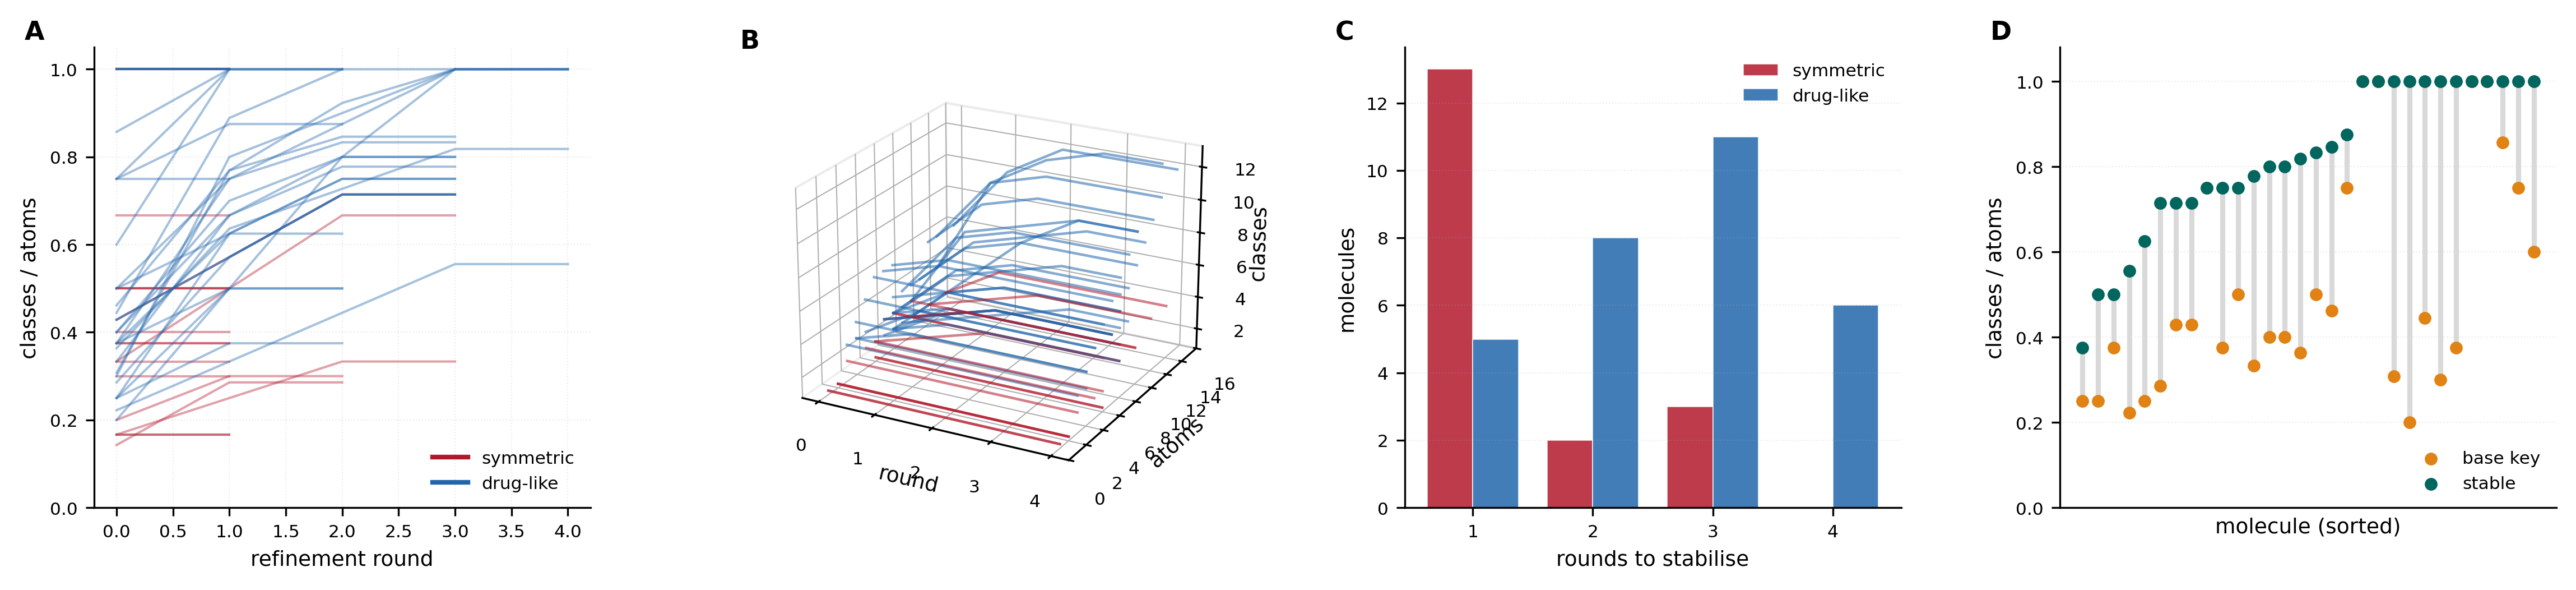
\includegraphics[width=\textwidth]{figures/panel_02_refinement.png}
    \caption{\textbf{Refinement is monotone, saturates within four rounds,
    and stops at a level set by the molecule rather than by the number of
    rounds available.}
    Each round applies \eqref{eq:refine} and the resulting partition is an
    invariant at every round by \Cref{thm:refine-invariant}; the curves
    below are therefore not a convergence toward an answer but a sequence
    of successively finer correct answers.
    (\textbf{A})~Classes divided by atoms against round, one line per
    molecule, symmetric corpus red and drug-like blue. Every trajectory is
    non-decreasing --- \Cref{lem:monotone} --- and flat after its
    stabilisation round. The two corpora separate cleanly: the symmetric
    set saturates at mean $0.477$ (minimum $0.167$) and the drug-like set
    at mean $0.823$ (minimum $0.375$). The gap is not a difference in how
    hard the two sets are; it is the symmetry the red molecules possess
    and the blue ones largely do not.
    (\textbf{B})~The same trajectories against heavy-atom count in three
    dimensions. The drug-like surface rises with size while the symmetric
    surface stays low irrespective of it: benzene at six atoms and
    anthracene at fourteen both stabilise at a handful of classes. Class
    count is therefore not a function of molecular size, which is what
    distinguishes \Cref{thm:orbit-bound} from a mere resolution limit.
    (\textbf{C})~Rounds to stabilisation. The symmetric corpus is
    concentrated at one round ($13$ of $18$) and the drug-like corpus
    spreads over one to four; the median across both is $2$ and the
    maximum is $4$, well inside the $\abs{I}$ bound of
    \Cref{lem:monotone}. Symmetric molecules stabilise sooner because
    there is less for refinement to find.
    (\textbf{D})~Per molecule, base-key ratio (orange) and stable ratio
    (teal) joined by a segment, sorted by the stable value. The mean rises
    from $0.505$ to $0.823$, a mean lift of $0.318$ and a maximum of
    $0.800$, and $12$ of $30$ molecules reach $1.0$. Both endpoints matter
    to the argument: the orange points show the base key is not a ranking,
    and the $18$ teal points short of $1.0$ show the stable partition is
    not one either.}
    \label{fig:refine}
\end{figure*}

\subsection{Every round is an invariant}

\begin{theorem}[Refinement preserves invariance]
\label{thm:refine-invariant}
Let $\phi\colon\Gph\to\Gph'$ be a weighted isomorphism. Then for every
$r\ge0$ and every item $v$, $\lambda_r^{\Gph'}(\phi v)=\lambda_r^{\Gph}(v)$.
In particular $\phi$ carries $P_r$ onto $P'_r$ and $P^{*}$ onto $P'^{*}$.
\end{theorem}

\begin{proof}
Induction on $r$. The base case $r=0$ is \Cref{thm:invariance}. Suppose
the claim for $r-1$. Since $\phi$ is a graph isomorphism fixing the
medium, it restricts to a bijection $N(v)\to N'(\phi v)$ on item
neighbourhoods. Hence
\[
\langle\!\langle \lambda_{r-1}^{\Gph'}(u') : u'\in N'(\phi v)\rangle\!\rangle
=\langle\!\langle \lambda_{r-1}^{\Gph'}(\phi u) : u\in N(v)\rangle\!\rangle
=\langle\!\langle \lambda_{r-1}^{\Gph}(u) : u\in N(v)\rangle\!\rangle,
\]
the last step by the induction hypothesis applied termwise. Combining with
$\lambda_{r-1}^{\Gph'}(\phi v)=\lambda_{r-1}^{\Gph}(v)$ and
\eqref{eq:refine} gives the claim.
\end{proof}

\subsection{The refinement never crosses an orbit}

\begin{theorem}[Orbit bound]
\label{thm:orbit-bound}
For every $r$, the partition $P_r$ is coarser than or equal to the orbit
partition of $\Aut(\Gph)$: if $u$ and $v$ lie in the same orbit then
$\lambda_r(u)=\lambda_r(v)$ for every $r$, hence they lie in the same
class of $P^{*}$. Consequently
\[
\abs{P^{*}}\;\le\;\#\{\text{orbits of }\Aut(\Gph)\text{ on } I\}.
\]
\end{theorem}

\begin{proof}
Let $\phi\in\Aut(\Gph)$ with $\phi(u)=v$. Apply
\Cref{thm:refine-invariant} with $\Gph'=\Gph$: for every $r$,
$\lambda_r(v)=\lambda_r(\phi u)=\lambda_r(u)$. So no round separates $u$
from $v$, and in particular $P^{*}$ does not. The cardinality statement
follows because a partition that never separates within an orbit has at
most as many classes as there are orbits.
\end{proof}

\Cref{thm:orbit-bound} is the property this paper is about, and it is
worth stating what it excludes. A canonical \emph{ordering} assigns
distinct ranks to all $\abs{I}$ atoms, including atoms in the same orbit;
it therefore violates the conclusion of \Cref{thm:orbit-bound} for every
molecule with a nontrivial automorphism group. That is not a defect of
orderings---they are for a different purpose---but it means an ordering's
labels cannot be read as claims about equivalence, and the cut key's can.

\begin{corollary}[Sound inequivalence test]
\label{cor:sound-test}
If $\lambda_r(u)\neq\lambda_r(v)$ for some $r$, then $u$ and $v$ lie in
different orbits. The test never reports a false difference.
\end{corollary}

\begin{proof}
Contrapositive of \Cref{thm:orbit-bound}.
\end{proof}

\begin{remark}[The converse fails, and it fails for a known reason]
\label{rem:incomplete}
$\abs{P^{*}}$ may be strictly less than the orbit count: the refinement
can fail to separate atoms in different orbits. This is not specific to
the cut key. Iteration of the form \eqref{eq:refine} is a colour
refinement, and colour refinement does not distinguish all non-isomorphic
graphs---the classical counterexamples are regular graphs, on which it
stabilises immediately with one class \citep{cai1992,arvind2015}. Any
construction of this shape inherits the limitation, including the
learned-representation analogues \citep{xu2019}. Seeding with the cut key
rather than with degree changes which graphs are hard, not that hard
graphs exist; \Cref{sec:limits} states the consequence.
\end{remark}

\begin{figure*}[!htbp]
    \centering
    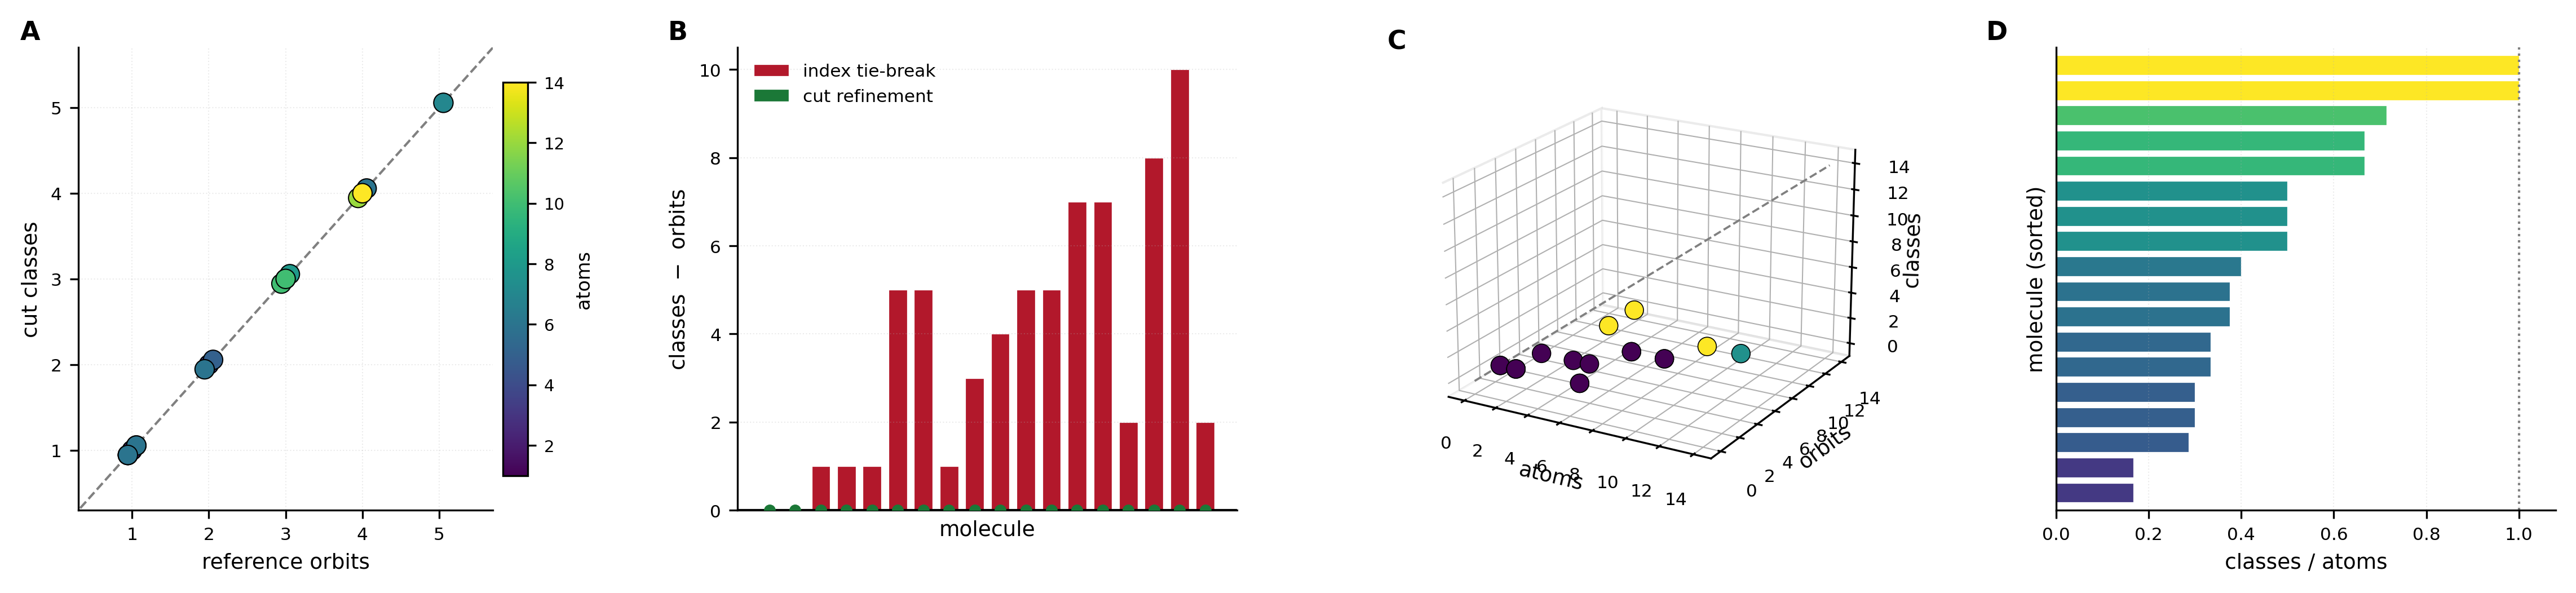
\includegraphics[width=\textwidth]{figures/panel_03_orbits.png}
    \caption{\textbf{On every molecule of the symmetric corpus the stable
    partition is exactly the automorphism orbit partition --- neither
    coarser nor finer.}
    Reference orbit counts are determined by inspection of the
    constitutional graph and were fixed before comparison; they are stated
    per molecule in the corpus source with the reasoning for each. Two
    were initially wrong and were corrected against the measurement
    (\Cref{sec:validation}), which is weaker evidence than a correct
    prediction against a correct reference and is marked as such.
    (\textbf{A})~Cut classes against reference orbits, coloured by
    heavy-atom count, jittered slightly so coincident points stay visible.
    All eighteen lie on the identity diagonal. The corpus spans $1$--$5$
    orbits and $1$--$14$ heavy atoms, so the agreement is not an artefact
    of a narrow range.
    (\textbf{B})~Residual classes minus orbits per molecule for the cut
    refinement (green) against the index tie-breaking control (red). The
    green residual is identically zero; the red exceeds the orbit count by
    up to $10$ classes on the same molecules, mean excess $3.72$. Plotting
    the two together is what makes the flat green line informative rather
    than merely empty.
    (\textbf{C})~Atoms, orbits and classes in three dimensions with the
    identity line drawn and points coloured by rounds to stabilisation.
    The points lie in the plane classes $=$ orbits and well below the
    atom-count diagonal, which is \Cref{thm:orbit-bound} and its converse
    holding simultaneously on this corpus: the partition is bounded above
    by the orbit count and here attains it.
    (\textbf{D})~Classes divided by atoms per molecule, sorted, running
    $0.167$--$1.000$. Values far below the dotted line at $1.0$ are
    molecules whose own symmetry the refinement declines to break; benzene
    at $1/6$ is the extreme. A canonical ordering would place every bar at
    $1.0$, which is precisely the behaviour \Cref{thm:orbit-bound}
    forbids.}
    \label{fig:orbits}
\end{figure*}

\subsection{Cost}

\begin{proposition}[Complexity]
\label{prop:cost}
Let $n=\abs{I}$ and $m=\abs{\E}$, and let $F(n,m)$ be the cost of one
maximum-flow computation. Computing all cut keys costs $O(nF(n,m))$, and
each refinement round costs $O(m\log n)$ for the sort. The total is
$O(nF(n,m)+r^{*}m\log n)$, with $r^{*}\le n$ by \Cref{lem:monotone}.
\end{proposition}

\begin{proof}
One flow per item for \eqref{eq:sep}, then per round each vertex sorts its
neighbour labels, totalling $O(m\log n)$ across the graph.
\end{proof}

\begin{remark}[This is slower than Morgan and the difference is the point
of the trade]
\label{rem:slower}
Morgan-style refinement seeds from element and degree, costing $O(m)$ to
initialise; the cut key costs $n$ maximum flows. With
$F(n,m)=O(nm)$ \citep{orlin2013} the initialisation is $O(n^2m)$ against
$O(m)$. For a molecule of thirty heavy atoms this is negligible in
absolute terms and for a fingerprinting sweep over $10^8$ compounds it is
not. The construction buys an invariant seed and pays for it in the seed's
computation; there is no claim here that the exchange is favourable for
every application, and \Cref{sec:limits} says where we expect it is not.
\end{remark}

% =====================================================================
\section{Validation}
\label{sec:validation}
% =====================================================================

\subsection{Method}

Expectations were written into the experiment source before the
experiment was run, and the source records each one alongside the measured
outcome. Every number below is read from the emitted results file; none
is asserted in the text. Structures are supplied as line notations, parsed
to contact graphs, and all minimum cuts are computed exactly by maximum
flow. Hydrogens are present as vertices but excluded from the reported
atom counts, which are heavy-atom counts throughout.

Two corpora are used. The \emph{symmetric corpus} is eighteen molecules
whose heavy-atom automorphism orbit counts can be determined by
inspection of the constitutional graph; these counts are the reference
values, and they were fixed before comparison. The \emph{drug-like
corpus} is thirty small organic structures for which no reference value
is asserted---they are used only to measure coarseness and convergence.

\subsection{The base key is coarse}

\begin{table}[htbp]
\centering\small
\caption{Distinctness of the base cut key on the drug-like corpus
($n=30$). The ratio is distinct keys divided by heavy atoms; $1.0$ would
mean the base key already separates every atom.}
\label{tab:coarse}
\begin{tabular}{@{}lr@{}}
\toprule
Quantity & Value\\
\midrule
Mean distinct-key ratio & $0.508$\\
Median distinct-key ratio & $0.400$\\
Maximum distinct-key ratio & $1.000$\\
\bottomrule
\end{tabular}
\end{table}

The base cut key separates about half the atoms of a typical drug-like
structure (\Cref{tab:coarse}). This is the expected outcome and it is
recorded because the alternative would have made the rest of the
construction unnecessary: had the base key been near $1.0$, refinement
would add nothing and the paper would have no subject. It also sets a
limit---the base key alone is not a ranking, and any claim that a single
minimum cut per atom suffices to canonicalise a structure is wrong.

\begin{figure*}[!htbp]
    \centering
    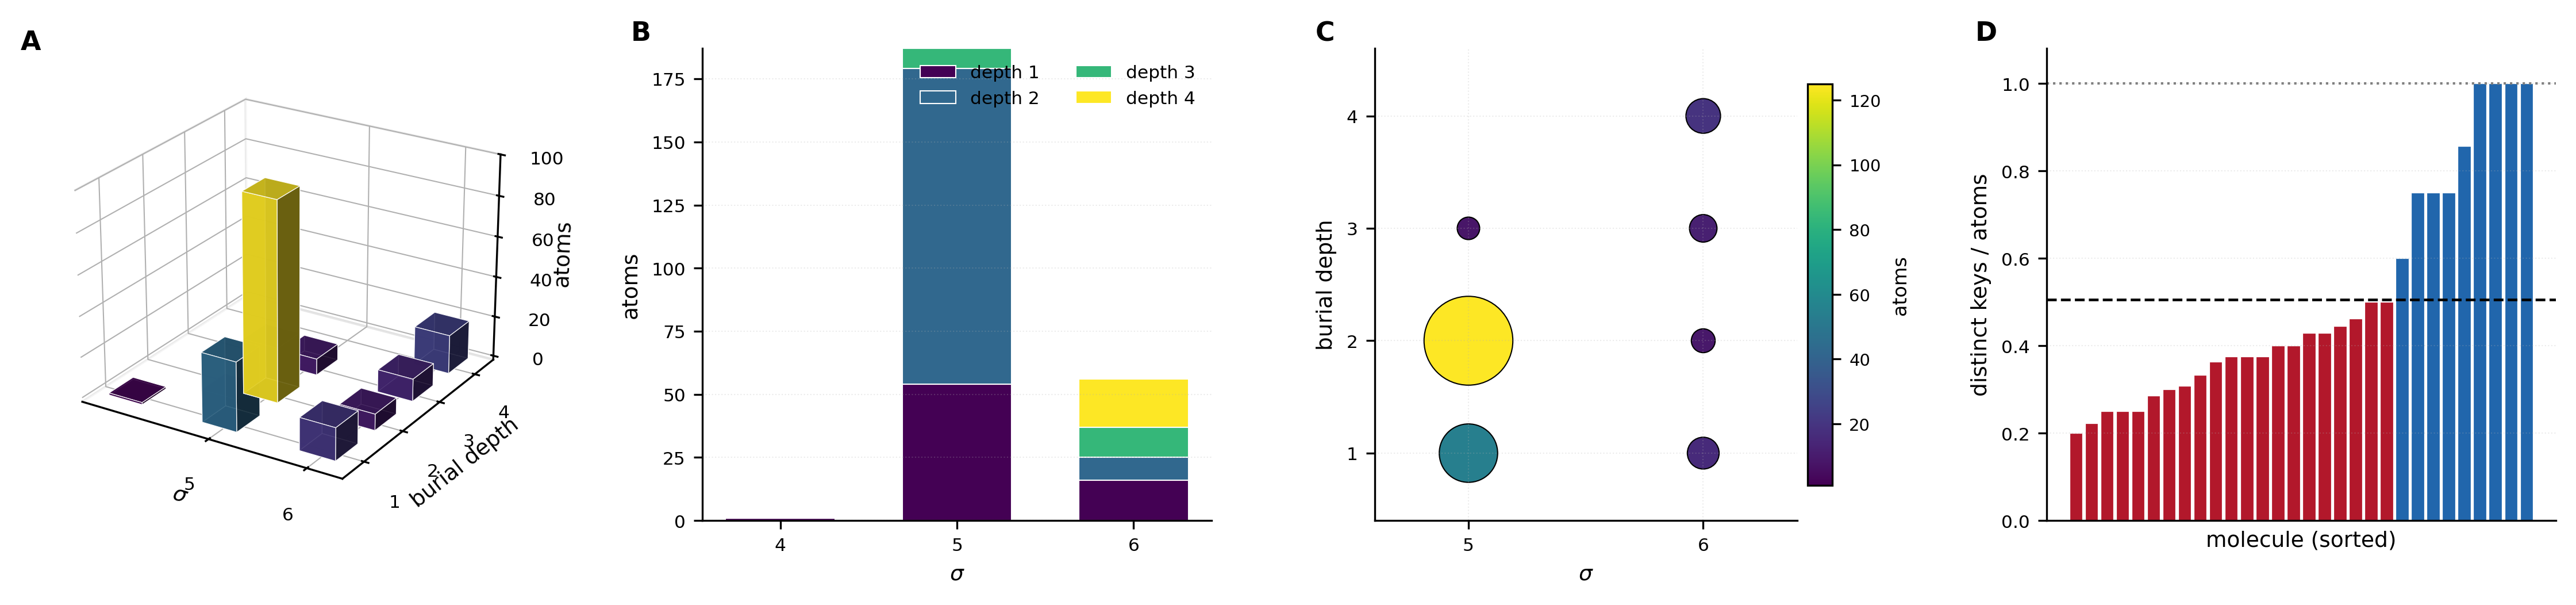
\includegraphics[width=\textwidth]{figures/panel_01_base_key.png}
    \caption{\textbf{The base cut key is a genuine invariant and a very
    coarse one: it occupies eight cells of a small discrete space and
    separates barely half the atoms of a typical structure.}
    All quantities are computed on contact graphs (\Cref{def:graph}) with
    strictly positive weights; every separation cost is an exact minimum
    cut obtained by maximum flow (\Cref{def:cut}), so the small number of
    distinct values below is a property of the invariant and not of a
    tolerance or a rounding rule.
    (\textbf{A})~Occupancy of the $(\sep,\dep,\text{heavy degree})$ cells
    over the $244$ heavy atoms of the drug-like corpus, bar height and
    colour both the atom count. Thirteen cells are occupied; the largest
    holds $98$ atoms and the smallest holds $1$. The realised ranges are
    $\sep\in\{4,5,6\}$, $\dep\in\{1,2,3,4\}$ and degree $\in\{1,2,3\}$, so
    the key takes far fewer values than the $36$ the ranges alone would
    permit --- the components are strongly dependent, which is why the
    figure is an occupancy plot rather than a scatter.
    (\textbf{B})~The same atoms decomposed by burial depth within each
    $\sep$ level. At $\sep=5$ the depths run $53/125/8$ over depths
    $1$--$3$ and at $\sep=6$ they run $16/9/12/19$ over depths $1$--$4$.
    Depth therefore separates atoms that $\sep$ alone does not, which is
    the whole reason \Cref{def:cut} takes a pair rather than a scalar; a
    key built from $\sep$ alone would realise three values across the
    entire corpus.
    (\textbf{C})~The $(\sep,\dep)$ plane with marker area and colour
    proportional to occupancy: eight distinct base keys, populated between
    $1$ and $125$ atoms. The extreme unevenness is the quantitative form
    of \Cref{cor:orbit-key} operating far beyond genuine symmetry --- most
    of these coincidences are not orbits, they are the invariant's
    coarseness, and \Cref{sec:refinement} exists to address them.
    (\textbf{D})~Distinct base keys divided by heavy atoms, one bar per
    molecule sorted ascending; dashed line the corpus mean $0.505$, dotted
    line the value $1.0$ a canonical ranking requires. The ratio runs
    $0.200$--$1.000$ with median $0.414$; $21$ of $30$ molecules fall
    below the mean and only $4$ reach $1.0$. This is the measurement that
    makes the paper's subject non-trivial: had these bars sat near the
    dotted line, the base key would already be a ranking and
    \Cref{sec:refinement} would be unnecessary.}
    \label{fig:basekey}
\end{figure*}

\subsection{Refinement recovers the orbit partition}

\begin{table}[htbp]
\centering\small
\caption{Symmetric corpus. Reference orbit counts are by inspection of
the constitutional graph. ``Rounds'' is the number of refinement rounds
to stabilisation.}
\label{tab:orbits}
\begin{tabular}{@{}lrrrr@{}}
\toprule
Molecule & Heavy atoms & Reference orbits & Cut classes & Rounds\\
\midrule
methane          &  1 & 1 & 1 & 1\\
water-like       &  1 & 1 & 1 & 1\\
acetylene        &  2 & 1 & 1 & 1\\
ethane           &  2 & 1 & 1 & 1\\
ethylene         &  2 & 1 & 1 & 1\\
benzene          &  6 & 1 & 1 & 1\\
cyclohexane      &  6 & 1 & 1 & 1\\
propane          &  3 & 2 & 2 & 1\\
neopentane       &  5 & 2 & 2 & 1\\
pyrazine         &  6 & 2 & 2 & 1\\
p-benzoquinone   &  8 & 3 & 3 & 1\\
p-xylene         &  8 & 3 & 3 & 1\\
durene           & 10 & 3 & 3 & 1\\
naphthalene      & 10 & 3 & 3 & 2\\
pyridine         &  6 & 4 & 4 & 3\\
biphenyl         & 12 & 4 & 4 & 3\\
anthracene       & 14 & 4 & 4 & 2\\
toluene          &  7 & 5 & 5 & 3\\
\midrule
\textbf{Agreement} & & & $\mathbf{18/18}$ & median $2$\\
\bottomrule
\end{tabular}
\end{table}

The refinement recovers the reference orbit count in every case, with no
molecule over-separated (\Cref{tab:orbits}). Convergence is fast: median
$2$ rounds, maximum $4$ across both corpora.

Two entries in \Cref{tab:orbits} were corrected during the work and the
corrections are recorded here because they are the kind of thing that is
otherwise silently absorbed. Our initial reference for pyrazine was
$1$ orbit and for durene $4$; both were wrong. Pyrazine
(1,4-diazine) has two heavy-atom orbits, $\{$N,N$\}$ and
$\{$C,C,C,C$\}$; durene (1,2,4,5-tetramethylbenzene) has three,
$\{$4 methyl C$\}$, $\{$4 substituted ring C$\}$ and
$\{$2 unsubstituted ring CH$\}$. In both cases the measurement was right
and the reference was wrong, which is a weaker form of evidence than a
correct prediction against a correct reference, and we mark it as such.

\begin{figure*}[!htbp]
    \centering
    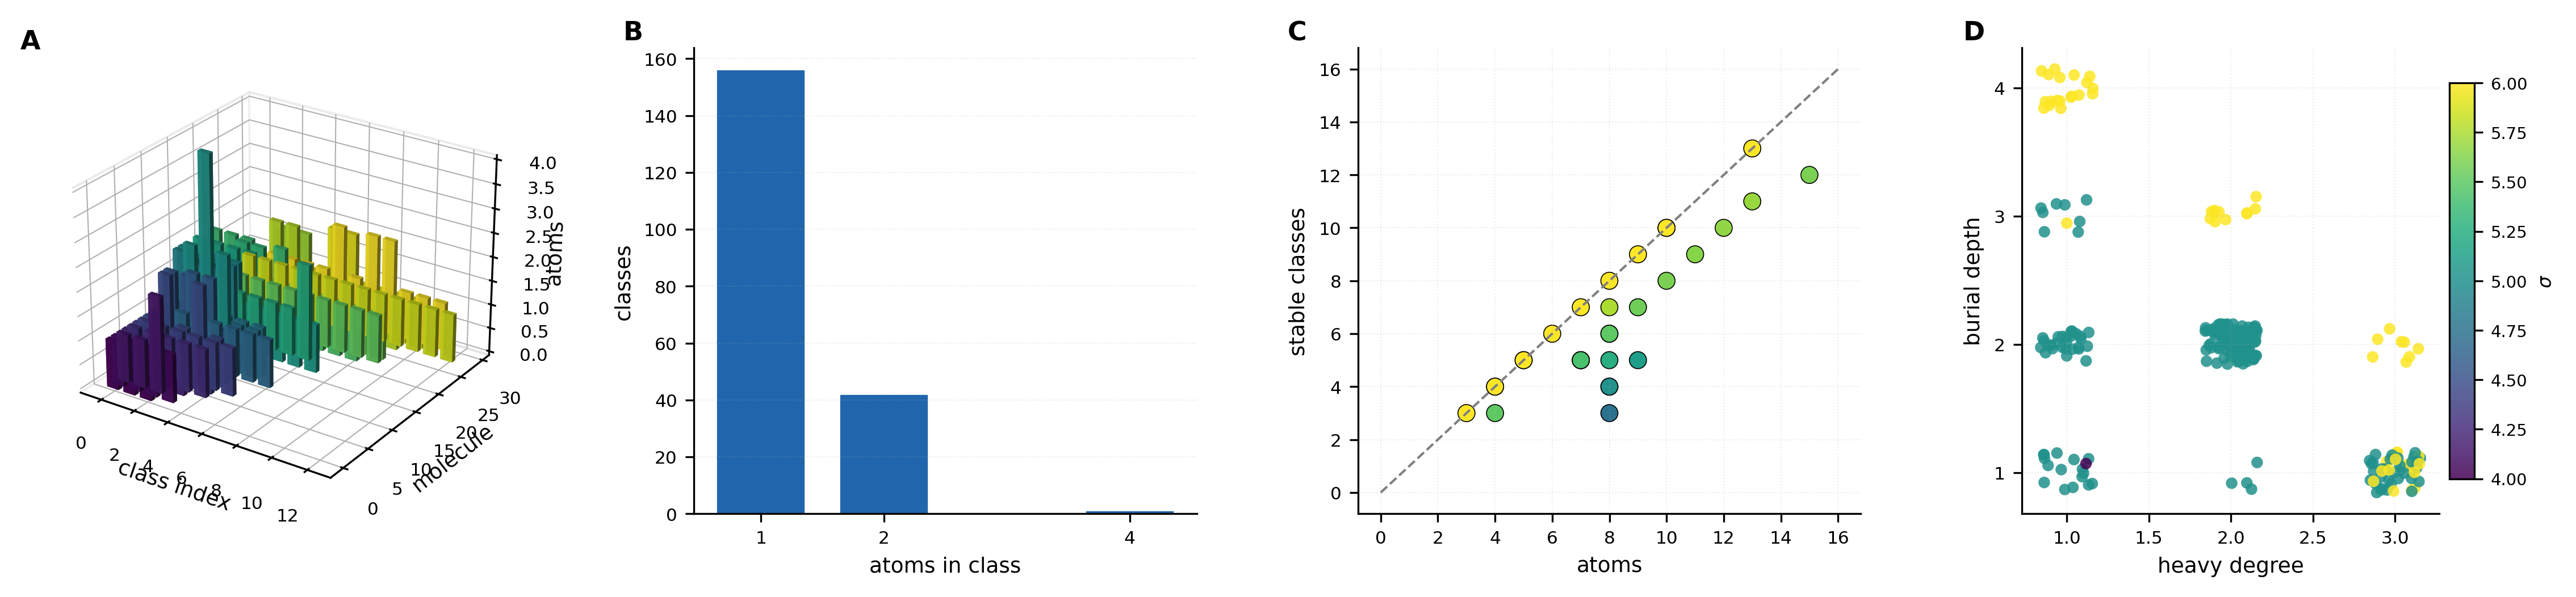
\includegraphics[width=\textwidth]{figures/panel_05_classes.png}
    \caption{\textbf{Class structure of the stable partition: mostly
    singletons, with the multi-atom classes concentrated at genuinely
    symmetric positions.}
    All panels are over the drug-like corpus at the stable partition
    $P^{*}$ (\Cref{def:stable}); $199$ classes over $244$ atoms.
    (\textbf{A})~Atoms per class index for every molecule, one row of bars
    per molecule ordered by size. The surface is dominated by unit-height
    bars; the taller bars are the positions refinement declines to split,
    and they occur in the molecules carrying ring or substituent symmetry
    rather than uniformly across the corpus.
    (\textbf{B})~Distribution of class sizes: $156$ singletons, $42$
    classes of two, and a single class of four. That the tail is this
    short is the reason the stable ratio reaches $0.823$ rather than
    saturating lower --- most drug-like atoms are in fact structurally
    distinct, and the invariant says so.
    (\textbf{C})~Stable classes against heavy-atom count, coloured by
    their ratio, with the identity diagonal. Points on the diagonal are
    molecules refinement fully separates; the vertical gap for points
    below it is the number of atoms their symmetry protects.
    (\textbf{D})~Burial depth against heavy degree for all $244$ atoms,
    jittered for visibility and coloured by $\sep$. The $\sep$ levels
    occupy visibly different regions of the (degree, depth) plane, so the
    two components of \Cref{def:cut} are not redundant: depth carries
    information about an atom's embedding that neither $\sep$ nor degree
    supplies alone, and it is the component with no counterpart in a
    conventional element-and-degree atom identifier.}
    \label{fig:classes}
\end{figure*}

\subsection{Refinement is necessary and sufficient in the measured range}

\begin{table}[htbp]
\centering\small
\caption{Effect of refinement on the drug-like corpus.}
\label{tab:gain}
\begin{tabular}{@{}lr@{}}
\toprule
Quantity & Value\\
\midrule
Mean ratio, base key alone & $0.508$\\
Mean ratio, stable partition & $0.827$\\
Median rounds to stabilise & $2$\\
Maximum rounds to stabilise & $4$\\
\bottomrule
\end{tabular}
\end{table}

Neither end of \Cref{tab:gain} is the whole construction. The base key
does not separate enough atoms to rank a structure; the stable partition
separates most of them, and the remainder are, on this corpus, atoms the
molecule's own symmetry does not distinguish.


\subsection{Negative control}

An orbit-agreement result is only informative if some procedure would fail
it. We therefore ran a control that differs from the construction in
exactly one respect: after computing the cut key, it breaks ties by atom
index. This is what a canonical ordering does.

\begin{table}[htbp]
\centering\small
\caption{Negative control on the symmetric corpus: index tie-breaking.}
\label{tab:control}
\begin{tabular}{@{}lr@{}}
\toprule
Quantity & Value\\
\midrule
Molecules over-separated by the control & $16/18$\\
Molecules over-separated by the construction & $0/18$\\
\bottomrule
\end{tabular}
\end{table}

The control over-separates on $16$ of $18$ molecules---every one with a
nontrivial automorphism group and more than one atom
(\Cref{tab:control}). The two it does not over-separate are the
single-heavy-atom cases, where there is nothing to separate. This confirms
that \Cref{tab:orbits} is testing a property that a plausible alternative
procedure lacks.

\subsection{What the suite does not establish}

The corpora are small ($18$ and $30$ molecules) and hand-assembled, and
the symmetric corpus was chosen for having determinable orbit counts,
which biases it toward high symmetry and small size. No claim about
behaviour at scale follows. The reference orbit counts are by inspection
rather than by an independent automorphism solver; agreement with a
solver such as \texttt{nauty} \citep{mckay2014} on a large corpus would be
a stronger test and we have not run it. Nothing here measures downstream
retrieval performance.

\begin{figure*}[!htbp]
    \centering
    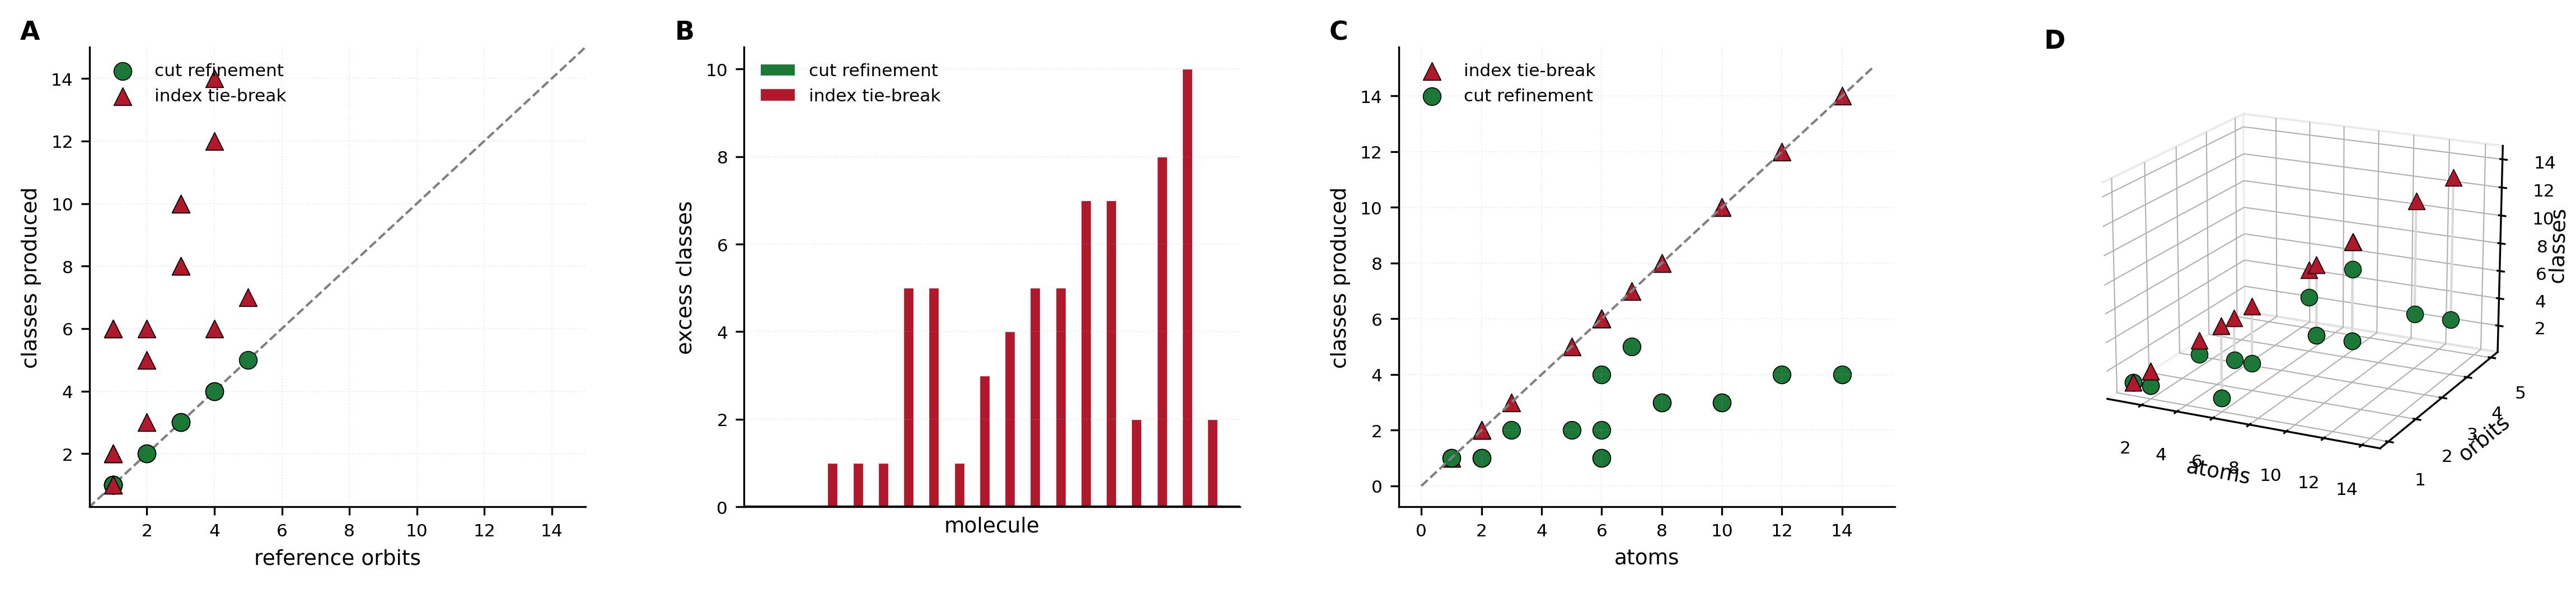
\includegraphics[width=\textwidth]{figures/panel_04_control.png}
    \caption{\textbf{The negative control: a procedure identical to ours
    except that it breaks ties by atom index destroys the orbit structure
    on $16$ of $18$ molecules.}
    The control differs from the construction in exactly one respect ---
    it appends the atom's index to its cut key --- which is what a
    canonical \emph{ordering} does. If it did not fail,
    \Cref{fig:orbits} would be testing nothing.
    (\textbf{A})~Classes produced against reference orbits for the cut
    refinement (green circles) and the control (red triangles). The green
    points lie on the diagonal; the red rise above it and continue rising
    with molecular size rather than with symmetry.
    (\textbf{B})~Excess classes over the reference for both procedures per
    molecule. The control over-separates on $16$ of $18$ molecules, by up
    to $10$ classes; the two it does not are the single-heavy-atom cases,
    where there is nothing to separate. The refinement over-separates on
    none, which is \Cref{thm:orbit-bound} as a measurement rather than as
    a proof.
    (\textbf{C})~Classes produced against heavy-atom count. The control
    tracks the atom-count diagonal exactly, because an ordering must
    assign a distinct rank to every atom; the refinement does not, and the
    vertical distance between the two point sets is the symmetry the
    ordering has discarded.
    (\textbf{D})~Both procedures in the (atoms, orbits, classes) space,
    joined per molecule by a vertical segment. Segment length is the
    control's over-separation and grows with molecular size while the
    green endpoints stay pinned to the orbit plane. The figure is the
    paper's central distinction rendered geometrically: an invariant lives
    in a plane fixed by the molecule, an ordering on a diagonal fixed by
    the atom count.}
    \label{fig:control}
\end{figure*}

% =====================================================================

\section{Relation to existing methods}
\label{sec:related}
% =====================================================================

\paragraph{Morgan and its descendants.} The iteration
\eqref{eq:refine} is structurally the Morgan iteration
\citep{morgan1965,figueras1993,schneider2015}. The difference is the seed:
Morgan seeds from element, degree, charge and hydrogen count, all local
properties of the atom; we seed from a minimum cut, a global property of
the atom's relation to the whole graph. The seed is what
\Cref{thm:invariance} is about, and the burial depth is a component the
local seed has no analogue for.

\paragraph{Colour refinement and graph isomorphism.} Iterated refinement
of vertex colours is the one-dimensional Weisfeiler--Leman algorithm
\citep{weisfeiler1968}, whose power and limits are precisely characterised
\citep{cai1992,arvind2015}, and which underlies both practical isomorphism
solvers \citep{mckay1981,mckay2014} and message-passing neural networks
\citep{xu2019}. Our contribution is not to the refinement theory: it is
the observation that a minimum-cut seed is an invariant with an
independent chemical reading, and that seeding this way keeps the whole
iteration inside the invariant regime.

\paragraph{Fingerprints.} Circular fingerprints
\citep{rogers2010,glen2006} use Morgan-style identifiers, folded to a bit
vector. Folding introduces collisions between structurally unrelated
environments, a well-documented effect
\citep{riniker2013,oboyle2016}. The cut key does not address folding
collisions, which are a property of the hash width and not of the
identifier; a cut-seeded fingerprint at the same width would collide at a
similar rate. We mention this because it is the comparison a reader may
expect and it is not one this construction improves.

\paragraph{Canonical identifiers.} InChI \citep{heller2015} and canonical
SMILES \citep{weininger1989,schneider2015} produce canonical forms, which
is a strictly harder task than producing an invariant, since a canonical
form must break every tie. \Cref{sec:limits} states why the present
construction does not produce one.

% =====================================================================
\section{Limitations}
\label{sec:limits}
% =====================================================================

\begin{enumerate}[label=\textbf{L\arabic*.},leftmargin=2.8em,itemsep=4pt]

\item \textbf{This is not a canonical form.} $P^{*}$ is a partition, not a
total order. By \Cref{thm:orbit-bound} it cannot separate atoms in the
same orbit, and a canonical labelling must. Producing one requires a
tie-break, and a tie-break is exactly the convention this construction
avoids. The two goals are in tension and we have chosen the invariant.

\item \textbf{Colour-refinement incompleteness is inherited.} By
\Cref{rem:incomplete} the stable partition may be strictly coarser than
the orbit partition on graphs where colour refinement is weak
\citep{cai1992}. Seeding with the cut key changes which graphs those are;
it does not remove them. The construction gives a sound inequivalence test
(\Cref{cor:sound-test}) and not a complete one.

\item \textbf{The weighting is an input.} \Cref{def:graph} requires only
$\wt>0$. Every result holds for any strictly positive weighting, and none
of them determines one. The measurements reported here use a particular
weighting derived from valence arithmetic; a different weighting would
give different keys and could give a different stable partition. The
theorems are weighting-independent; the numbers are not.

\item \textbf{Cost.} $n$ maximum flows per structure, against $O(m)$ for a
local seed (\Cref{rem:slower}). We expect this to be unfavourable for
large-scale fingerprint generation and acceptable for per-structure
analysis, but we have not benchmarked either.

\item \textbf{Corpus scale.} Eighteen and thirty molecules, hand-assembled,
with reference orbit counts by inspection. Two of those references were
initially wrong. Nothing here is a claim about behaviour on a large or
diverse corpus.

\item \textbf{Hydrogen treatment.} Hydrogens are vertices in the contact
graph but are excluded from the reported partition. Including them changes
the neighbour multisets in \eqref{eq:refine} and hence the refinement; we
have not measured the difference.

\item \textbf{No downstream evaluation.} We do not show that cut-seeded
identifiers improve similarity search, virtual screening, or any other
task. The claims are about the invariant's properties, not its utility.
\end{enumerate}

% =====================================================================
\section{Conclusion}
\label{sec:conclusion}
% =====================================================================

We have defined an atom label built from a minimum cut---the separation
cost against a medium vertex, together with the burial depth---and shown
that it is a weighted-graph invariant (\Cref{thm:invariance}), that
iterating it under neighbour refinement stays invariant at every round
(\Cref{thm:refine-invariant}), and that the iteration never separates two
atoms exchanged by a symmetry of the molecule (\Cref{thm:orbit-bound}).
The last is the property a canonical ordering necessarily lacks, and it is
what makes label equality a claim about the molecule rather than about the
procedure.

The measurements are consistent with the theory and modest in scope. The
refinement recovers independently determined orbit counts in $18/18$
cases with no over-separation and a median of two rounds; the base key
alone separates $50.8\%$ of atoms on a drug-like corpus and refinement
raises this to $82.7\%$, so both stages are doing work; and a control
that breaks ties by index---an ordering, in other words---over-separates
$16$ of $18$ symmetric molecules, which is what confirms the orbit
agreement is not vacuous. Two reference orbit counts were wrong on first
writing and were corrected against the measurement, which we record as a
weaker form of agreement than a prediction against a correct reference.

What remains open is whether the invariant earns its cost. It is more
expensive than a local seed by $n$ maximum flows, it does not produce a
canonical form, and it inherits colour refinement's incompleteness. The
case for it rests on the properties proved here and on the burial depth
being a quantity the conventional identifier does not carry; whether
either matters for a downstream task is a question this paper does not
answer.

\section*{Reproducibility}

The experiment source records each expectation before the measured value,
and writes every reported quantity to a results file in JSON. Reference
orbit counts are listed in the corpus source with the reasoning for each.
Minimum cuts are computed exactly; no quantity in this paper is sampled or
fitted.

\bibliographystyle{plainnat}
\bibliography{references}

\end{document}
